\documentclass{beamer}
\usetheme{Madrid}
\usecolortheme{beaver}

\logo{
\includegraphics[width=1cm]{1200px-King's_College_London_logo.svg.png}}

\title{Progress Slides I (5th Feb 24)}
\author{Oscar Moxon}
\institute{King's College London}

\begin{document}

\begin{frame}
\titlepage
\end{frame}

\begin{frame}
    \textbf{Contents:}
    \frametitle{Overview of Multi-Agent Debate Systems}
    \begin{itemize}
        \item Exploration of Multi-Agent Debate (MAD) systems to facilitate scientific inquiry dialogues [1].
        \vspace{5mm}
        \item Motivation: Integration of debate mechanics to enhance reasoning capabilities of language models [3, 4, 6].
        \vspace{5mm}
        \item Human-in-the-loop as a critical component for monitoring judgements and completing tasks requiring embodiment [8].
    \end{itemize}
\end{frame}

\begin{frame}
    \frametitle{Making New Discoveries with LLMs}
    \begin{columns}[T]
        \begin{column}{.48\textwidth}
            \textbf{LLMs and Scientific Discovery}
            \begin{itemize}
                \item Increasingly apparent that LLMs can produce novel insights about notorious scientific problems.
                \item Pairing of pretrained LLM with a systematic evaluator to iterate on solutions to the cap set problem.
                \item LLM generates constructions that are interpretable and falsifiable.
                \item Leads to the largest improvement in 20 years. 
            \end{itemize}
        \end{column}
        \hfill
        \begin{column}{.48\textwidth}
            \textbf{Refinement and Feedback Loop}
            \begin{itemize}
                \item Role of evaluator is to guard against confabulations and incorrect ideas.
                \item Best-shot prompting to enhance algorithms, creating a positive feedback circuit.
            \end{itemize}
            \begin{figure}
                \centering
                \includegraphics[width=0.9\textwidth]{FunSearch.png}
                \caption{FunSearch.}
            \end{figure}
        \end{column}
    \end{columns}
\end{frame}
    
\begin{frame}
    \frametitle{Capabilities of Autonomous Agents}
    \begin{columns}[T] % align columns
        \begin{column}{.48\textwidth}
            \begin{itemize}
                \item Web search capabilities are crucial for agents to process and synthesize current information.
                \item Fostering unique personas promotes specialization and varied viewpoints.
                \item Emphasis on specific expertise integrates diverse perspectives for richer outcomes.
                \item Human-like evaluation dynamics ensure adaptability and robust responses to novel information.
            \end{itemize}
        \end{column}
        \begin{column}{.48\textwidth}
            \begin{itemize}
                \item Agents’ multimodal abilities, such as those provided by Visual Transformers (ViT), enhance interaction fidelity.
            \end{itemize}
            \begin{figure}    
                \centering
                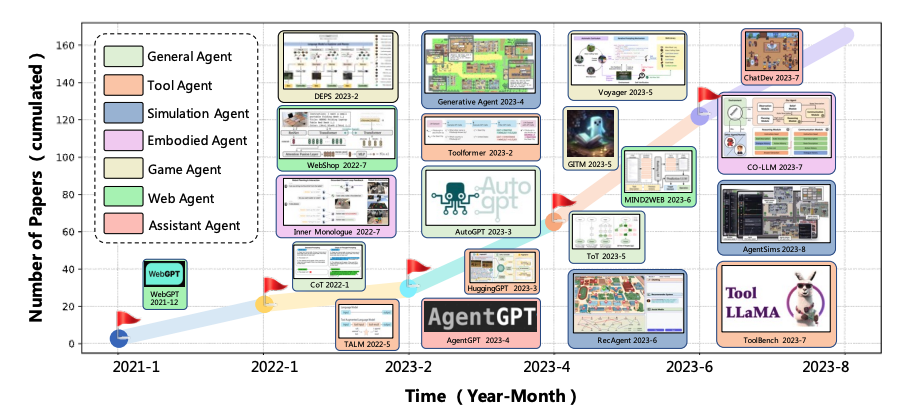
\includegraphics[width=\textwidth]{autonomous_agents.png}
                \caption{Map of Autonomous Agents Research in 2023.}
            \end{figure}
        \end{column}
    \end{columns}
    \end{frame}
    
\begin{frame}
    \frametitle{Reasoning and Debate Mechanics}
    
    \begin{columns}[T] % align columns
        \begin{column}{.5\textwidth}
            \textbf{}
            \begin{itemize}
                \item Giving agents the ability to self-reflect and Chain of Thought (CoT) enables advanced reasoning beyond one-shot prompts.
                \item Overcoming Degeneration-of-Thought (DoT) with feedback cycles for agent cross-evaluation.
                \item Formal debate dynamics through multiple rounds, with judging agent or voting protocol in place.
            \end{itemize}
        \end{column}
        \begin{column}{.5\textwidth}
            \textbf{}
            \begin{itemize}
                \item Embracing the Society of Minds concept.
                \item Collective intelligence factor significantly boosts reasoning in agent systems across benchmarks.
                \item Multi-Agent Debate (MAD) promotes divergent thinking.
            \end{itemize}
            \begin{figure}
                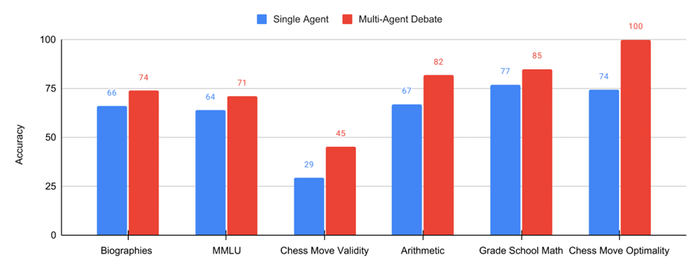
\includegraphics[width=0.8\textwidth]{debate_improvements.png}
            \end{figure}
        \end{column}
    \end{columns}
    \end{frame}
        

\begin{frame}
    \frametitle{Multi-Agent System for Debate and Inquiry}
    
    \begin{columns}[T] % align columns
        \begin{column}{.5\textwidth}
            \textbf{Project Objectives}
            \begin{itemize}
                \item Construct a multi-agent system framework aimed at simulating debate and inquiry processes to enhance knowledge discovery.
                \item Develop an interpretable process with a judge that evolves discussion productively.
                \item Equip agents with ability to evaluate research, supporting arguments or challenging opposing views.
                \item Enable human interaction to further positive feedback.
            \end{itemize}
        \end{column}
        \begin{column}{.5\textwidth}
            \textbf{Implementation Timeline}
            \begin{itemize}
                \item By 27th Feb: Have plan for implementing this system, supported by multi-agent debate papers and open source projects.
            \end{itemize}
            \vspace{1em} % Adjust space as needed
            \begin{figure}
                \centering
                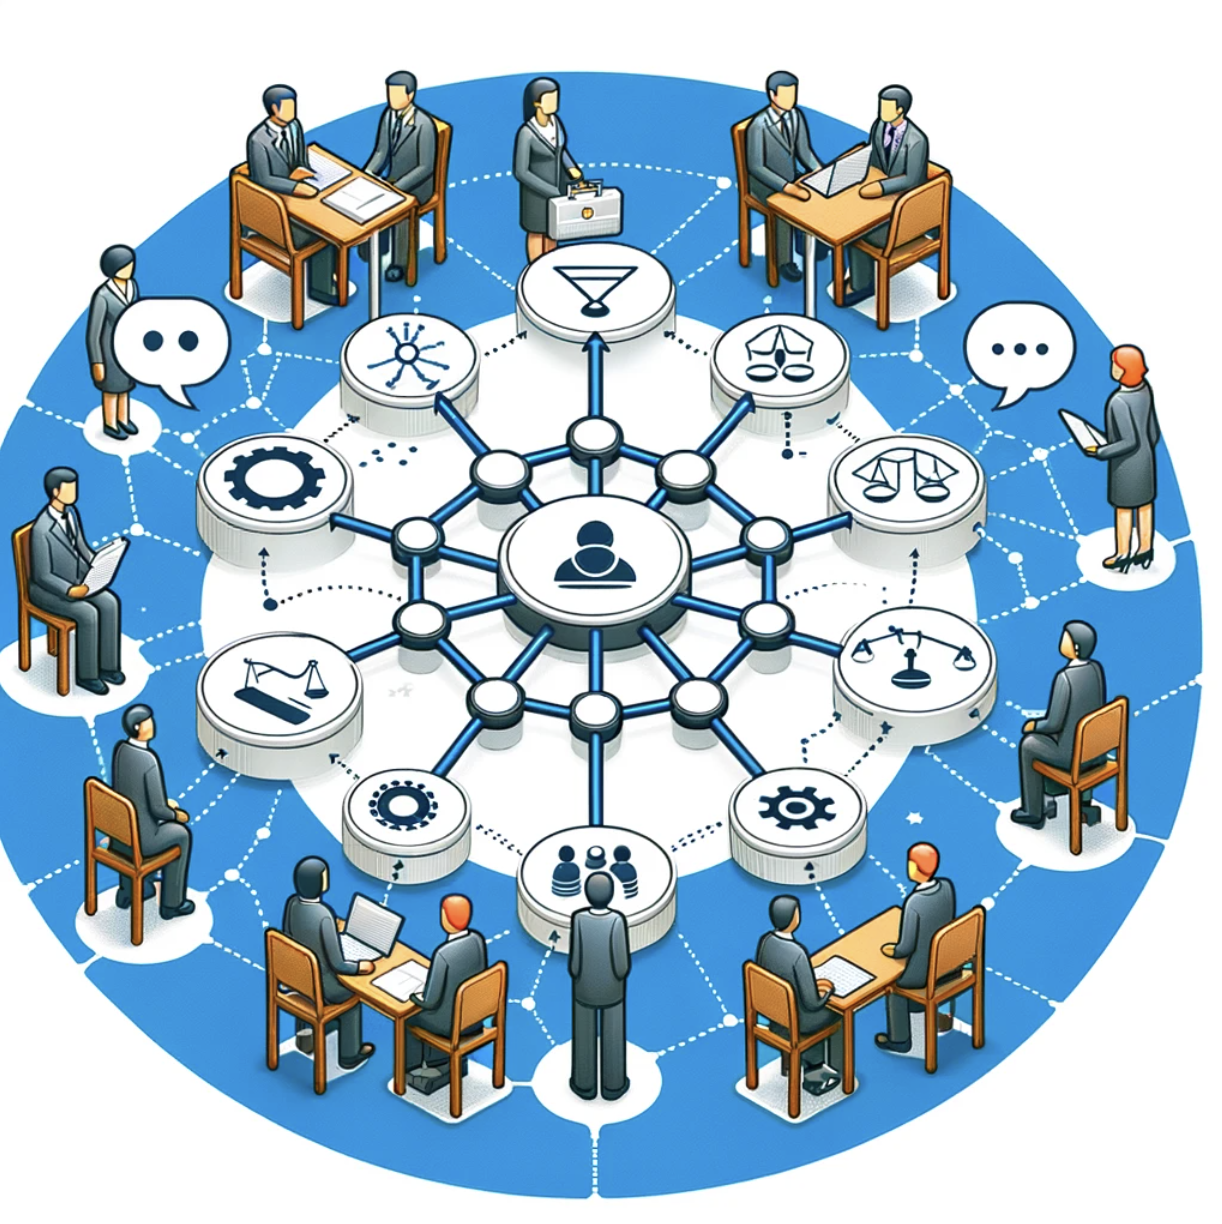
\includegraphics[width=\textwidth]{chatlab.png}
                \caption{}
            \end{figure}
        \end{column}
    \end{columns}
    
\end{frame}
        

\begin{frame}
\frametitle{Literature Overview}
\begin{enumerate}
    \item Encouraging Divergent Thinking in Large Language Models Through Multi-Agent Debate 
    \item A Survey on Large Language Model based Autonomous Agents
    \item Collective Intelligence Factor in Groups
    \item ChatEval: multi-agent debate towards better LLM-based evaluators
    \item FunSearch
    \item Igniting Language Intelligence
    \item Large Language Models Cannot Self-Correct Reasoning Yet
    \item The Rise and Potential of LLM Agents: A Survey
\end{enumerate}
\end{frame}

\end{document}
